%----------------Experimental Section-------------------------


%States the design requirements for the project
\subsection{Competition Requirements}

The NASA Student Launch Initiative \cite{NASA_SL} is a research-based competition partnered with NASA's Centennial Challenges, and aims to stimulate rapid, low-cost development of rocket propulsion and space exploration systems.  Both collegiate and non-academic teams participate in the 8-month competition cycle composed of design, fabrication, and testing of flight vehicles, payloads, and ground support equipment. 

The purpose of the 2014-2015 competition was to simulate a Mars Ascent Vehicle (MAV) and to perform a sample recovery from the Martian surface. The requirements for this simulation were twofold: (1) Design and deploy a system termed the Autonomous Ground Support Equipment (AGSE) that independently retrieves a sample off the ground and stores it in the payload bay of a rocket, and (2) launch the rocket to an altitude of 3000 ft. before safely recovering the sample. 

 %For this purpose, the mechanical design of the AGSE followed a modular, quick-to-build approach and ROSMOD was used for software development in order to quickly make on-the-fly adjustments to system behavior.


\subsection{AGSE Project Architecture}
%States how we meet those design requirements (related to the agse)
%components: robotic arm and payload bay "in order to accomplish X we used Y"
%robot behavior, workspace, and control
%payload bay behavior and design "controlled through serial port by agse, otherwise not part of the rosmod-based design process"
%state chart

The sample retrieval was accomplished using a robotic arm with computer vision to find the sample and identify its orientation. After successfully acquiring the sample, the system will then search for the payload bay, identify its orientation, and place the sample within it.  The robot arm itself is a simple crane-style device akin to a pick-and-place robot with a four-pronged gripper as the end effector.  It was designed to have a cylindrical workspace in order to most efficiently access the ground around the system and rocket. It starts in a known position and incrementally scans its workspace using a built in camera. Image processing is performed to identify key environmental features such as the sample and payload bay.

Sample retention was accomplished by implementing a motorized compartment within the nosecone of the rocket.  Upon receiving an "open" command from the AGSE a lead screw actuated system opens the nosecone, revealing a carbon fiber tray in which to place the sample. After successful operation of the AGSE, a "close" command is sent and the nose cone returns to its flight-ready configuration, sealing the sample in place.

While the driving requirements of the competition were fixed, many of the minor rules regarding AGSE performance, behavior, and safety requirements evolved and were augmented throughout the course of the competition. The volatile nature of these rules combined with the short eight month duration of the build cycle precipitated the need for rapidly adjustable design and fabrication processes. As such, an iterative, modular, design-build-test approach was implemented in order to concurrently develop as many components of the hardware and software systems as possible. An initial AGSE prototype was conceptualized from off-the-shelf components and the mechanical and software systems were built in parallel, integrated, and tested. These preliminary results were then used in future development to produce a more ideal structure with greater positional accuracy and system robustness.  Due to the modular nature of the system's design, it was not necessary to immediately build a completely new second system, so incremental improvements could be made on a specific subsystem (such as the robot's gripper, any single degree of freedom, image processing, motor control, etc.) as the design evolved.

%maybe too rambly between this paragraph and the last
One significant set of challenges to the construction of the AGSE were time, machinist skill level, and the facilities available to the group's workforce. The team consisted mainly of undergraduate workers with limited machining experience and no access to CNC machinery.  Due to this constraint, the mechanical design and software needed to accommodate generous tolerance allowances in component machining. The system also needed to be robust enough to recover from the failure of a component, such as that detailed in Performance Assessment.



\subsection{Mechanical Design}
%Details the design


\subsubsection{Kinematics}
%describe the joint structure of the robot, detail the coordinate system, etc.

The AGSE is a 4-DOF robot utilizing a revolute base joint to rotate the robot body, two prismatic joints to move vertically and horizontally, and a final revolute joint providing an orienting wrist for the end effector. A wireframe and workspace rendering of the AGSE can be seen in Figure \ref{fig:Render}.


\begin{figure}[h]
	\centering
	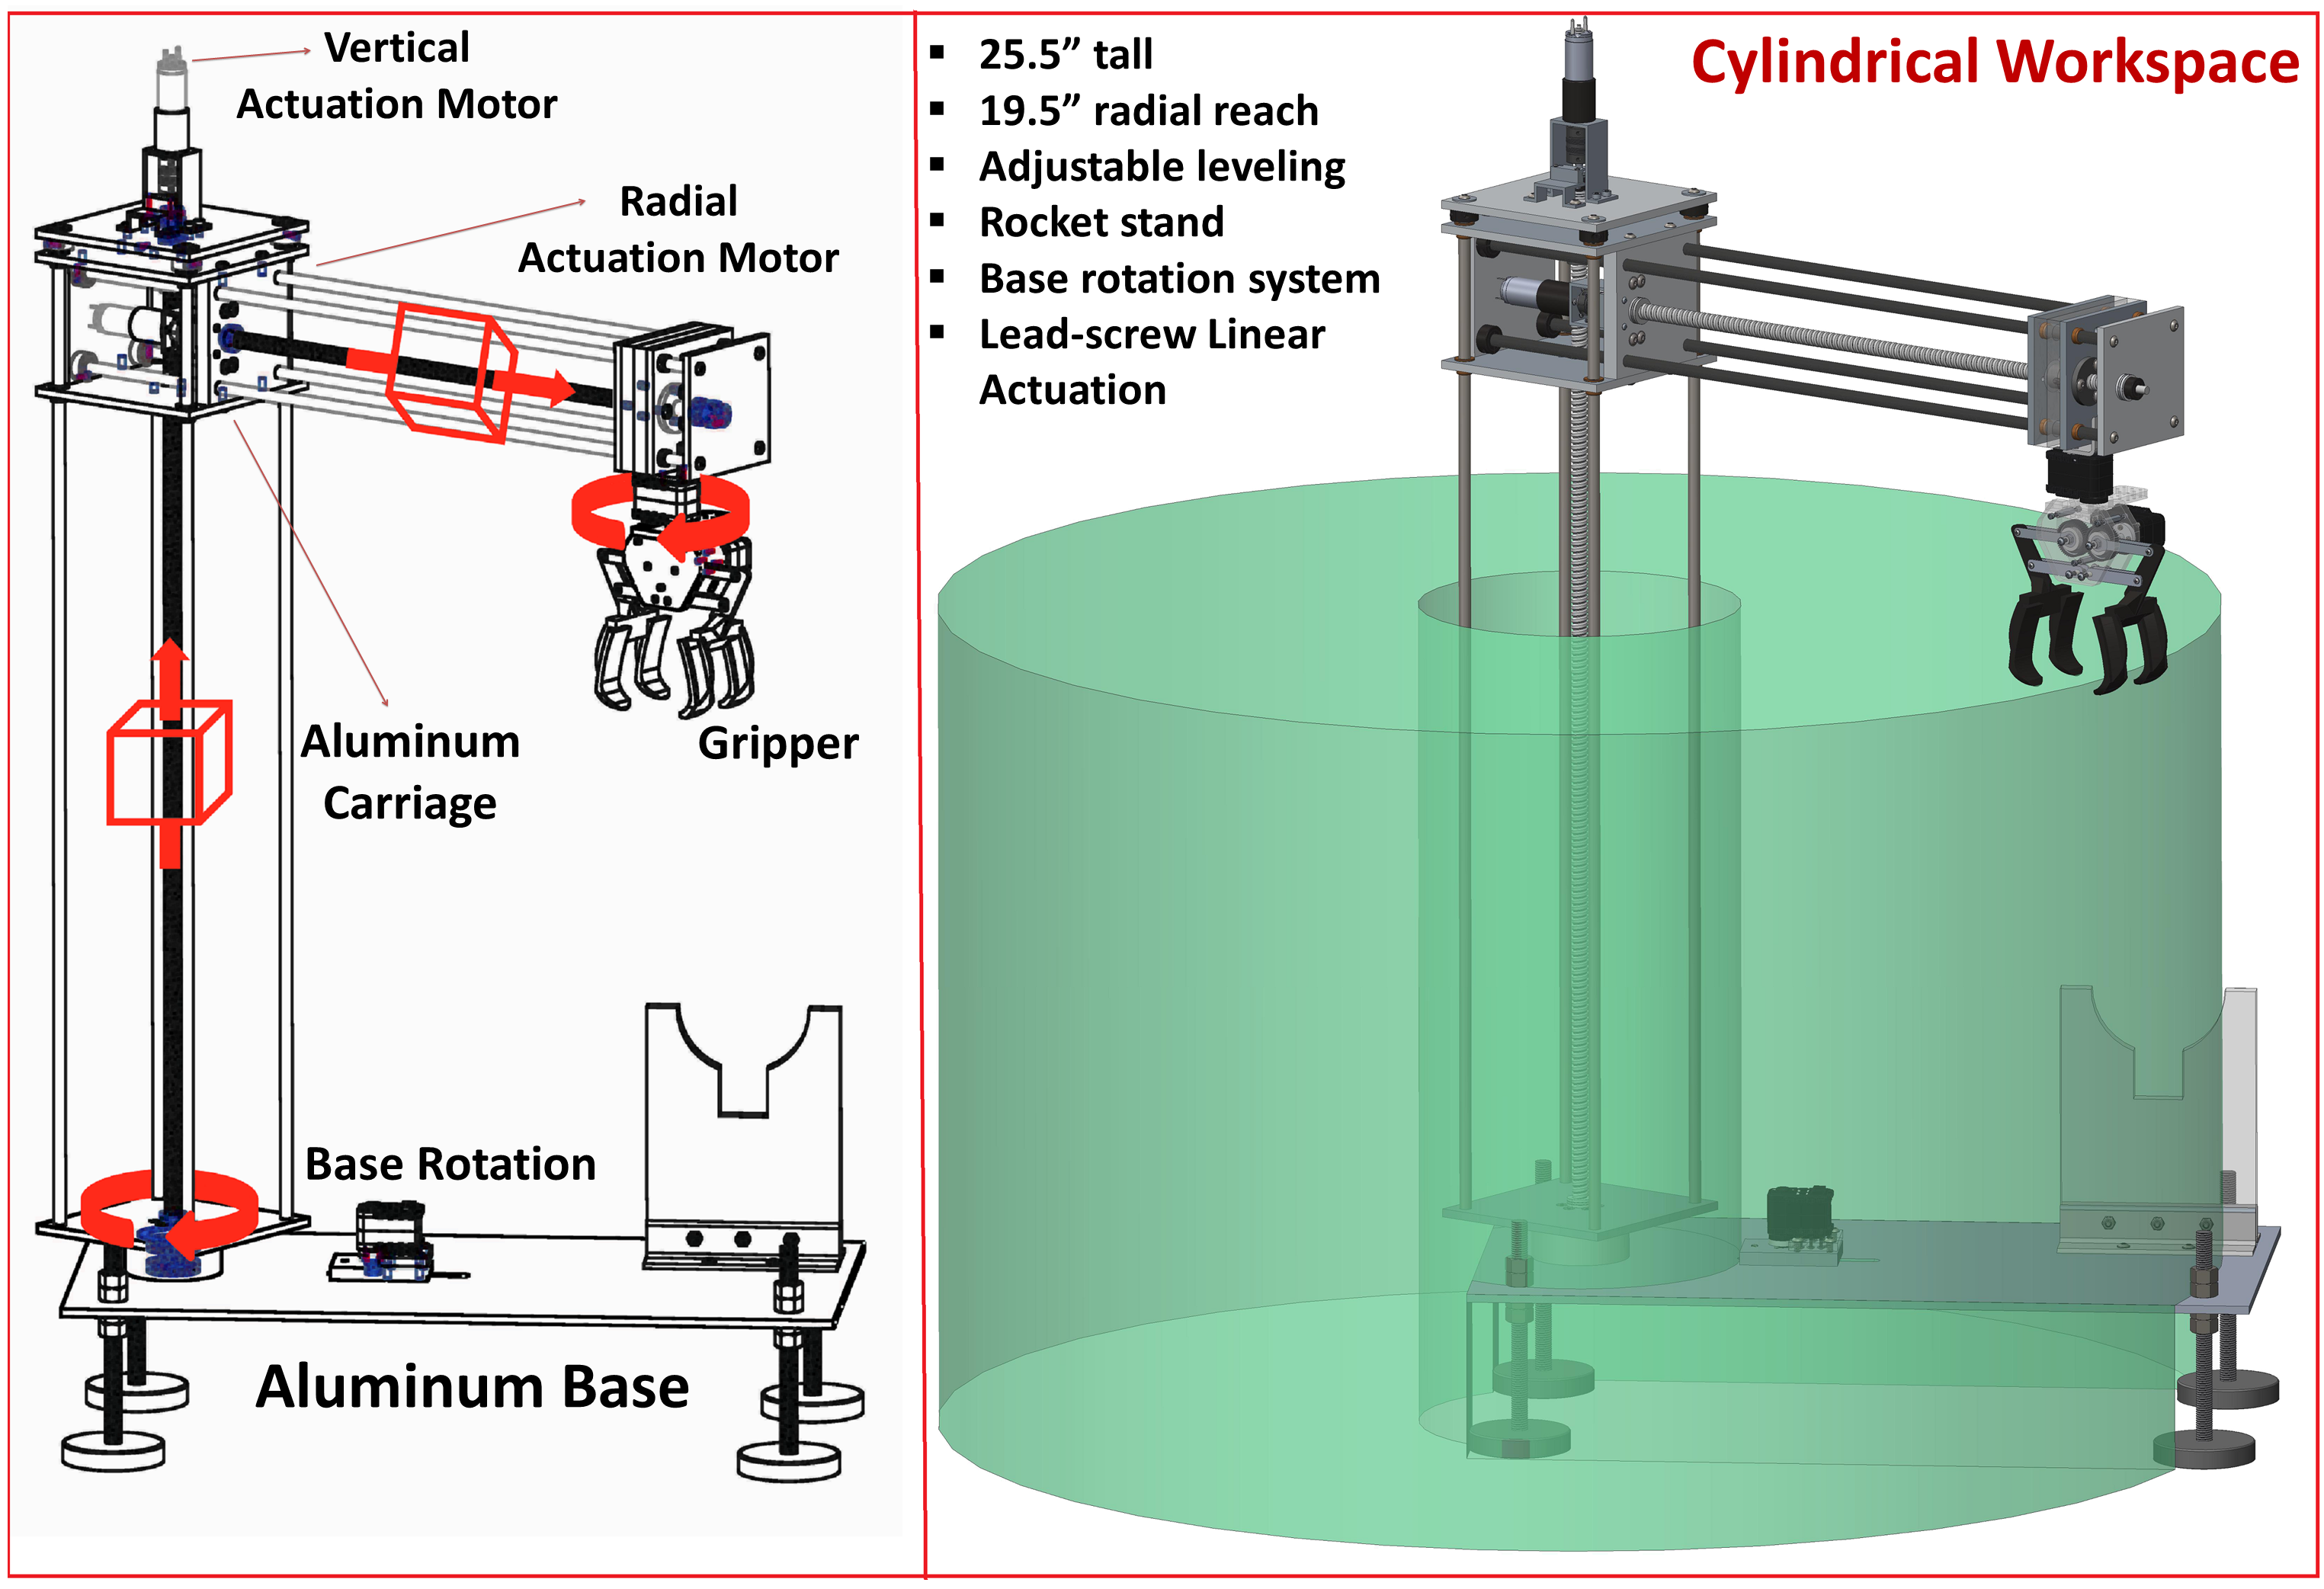
\includegraphics[width=0.48\textwidth]{figs/AGSE_Mechanical_Design_Figure.png}
	\caption{AGSE Mechanical Design}
	\label{fig:Render}
\end{figure}

%description of coordinate system
By design, the single revolute and two prismatic joints of the AGSE provide the basis for a cylindrical coordinate system and workspace, reducing the implementation of both forward and reverse kinematics to a trivial exercise of mapping joint position to the corresponding coordinate in the workspace. 

\begin{bmatrix}\boldsymbol{\theta}_{workspace}\\\mathbf{r}_{workspace}\\\mathbf{z}_{workspace}\end{bmatrix}=\begin{bmatrix}\boldsymbol{\theta}_{rev}\\\mathbf{r}_{pris}\\\mathbf{z}_{pris}\end{bmatrix}

%?equations of end-effector position based on joint posiiton?

\subsubsection{Structure}
%describe the physical structure of the base, each joint starting at the base, mounting hardware for electronics

The AGSE base is comprised of a machined sheet of aluminum upon which leveling legs are mounted to easily account for uneven surfaces.  Protruding from the base is the revolute joint, a machined spindle centered within ball bearing cup. Extending upwards along this rotational axis is the vertial join, a lead screw and guide rod assembly driving an aluminum carriage. A similar lead screw-carriage assembly extends from the side of the vertical carriage to provide motion within the horizontal plane. A mounting point for both the gripper and camera hangs from this horizontal carriage.

Underneath the base is a platform for mounting batteries, power regulation and protection circuitry, and onboard computer systems.  At the top of the vertical assembly is a mounting point for the actuator control electronics.


\subsubsection{Actuation and Sensing}
%detail the actuators used for each joint and all sensors utilized

A Dynamixel servo is mounted to the revolute joint's spindle to provide rotational movement. Two additional Dynamixel servos are used to orient and actuate the gripper. The two lead screw assemblies are driven using 12 volt Faulhaber motors mounted directly to the lead screws.

The AGSE guides the end effector motion using the limit switch-encoder combo on its linear actuators, the built in positional feedback from the servo motors, and the optical feedback provided by a camera mounted above the end effector (allowing the AGSE to recognize objects within the reachable area underneath the gripper phalanges).  Limit switches are mounted at the minimum and maximum of each lead screw assembly's range of movement, providing hard stops to motor actuation.  Quadrature encoders are then used within this range of motion to monitor the position of the vertical and horizontal carriages. The Dynamixel servos controlling the revolute joint and gripper provide position and speed feedback, as well as PID tuning to allow for quick and responsive control.


\subsection{Electrical Design}


\subsubsection{Power System}
%What powers it: Originally 2 12v batteries, now using power supply
%On/Off with relay
%Power Protection: Originally none, now have a fuse board
%


\subsubsection{Communication}
%How do the components communicate? Servos daisychained and identified by device ID and controled via modified dynamixel library, BBB, Jetson, and UIP connected to network with static IPs, etc.


\subsection{Control}
%Touch on these topics: Low-Level Motor Control, High-Level control  (Introduce image processing and path planning), feedback processing



\subsubsection{Distributed Deployment}

The AGSE robot is controlled by a distributed set of embedded controllers. Figure \ref{fig:AGSE_Deployment} shows the high-level design for the deployment architecture. There are three embedded devices, each with its own responsibilities. 

\begin{figure}[h]
	\centering
	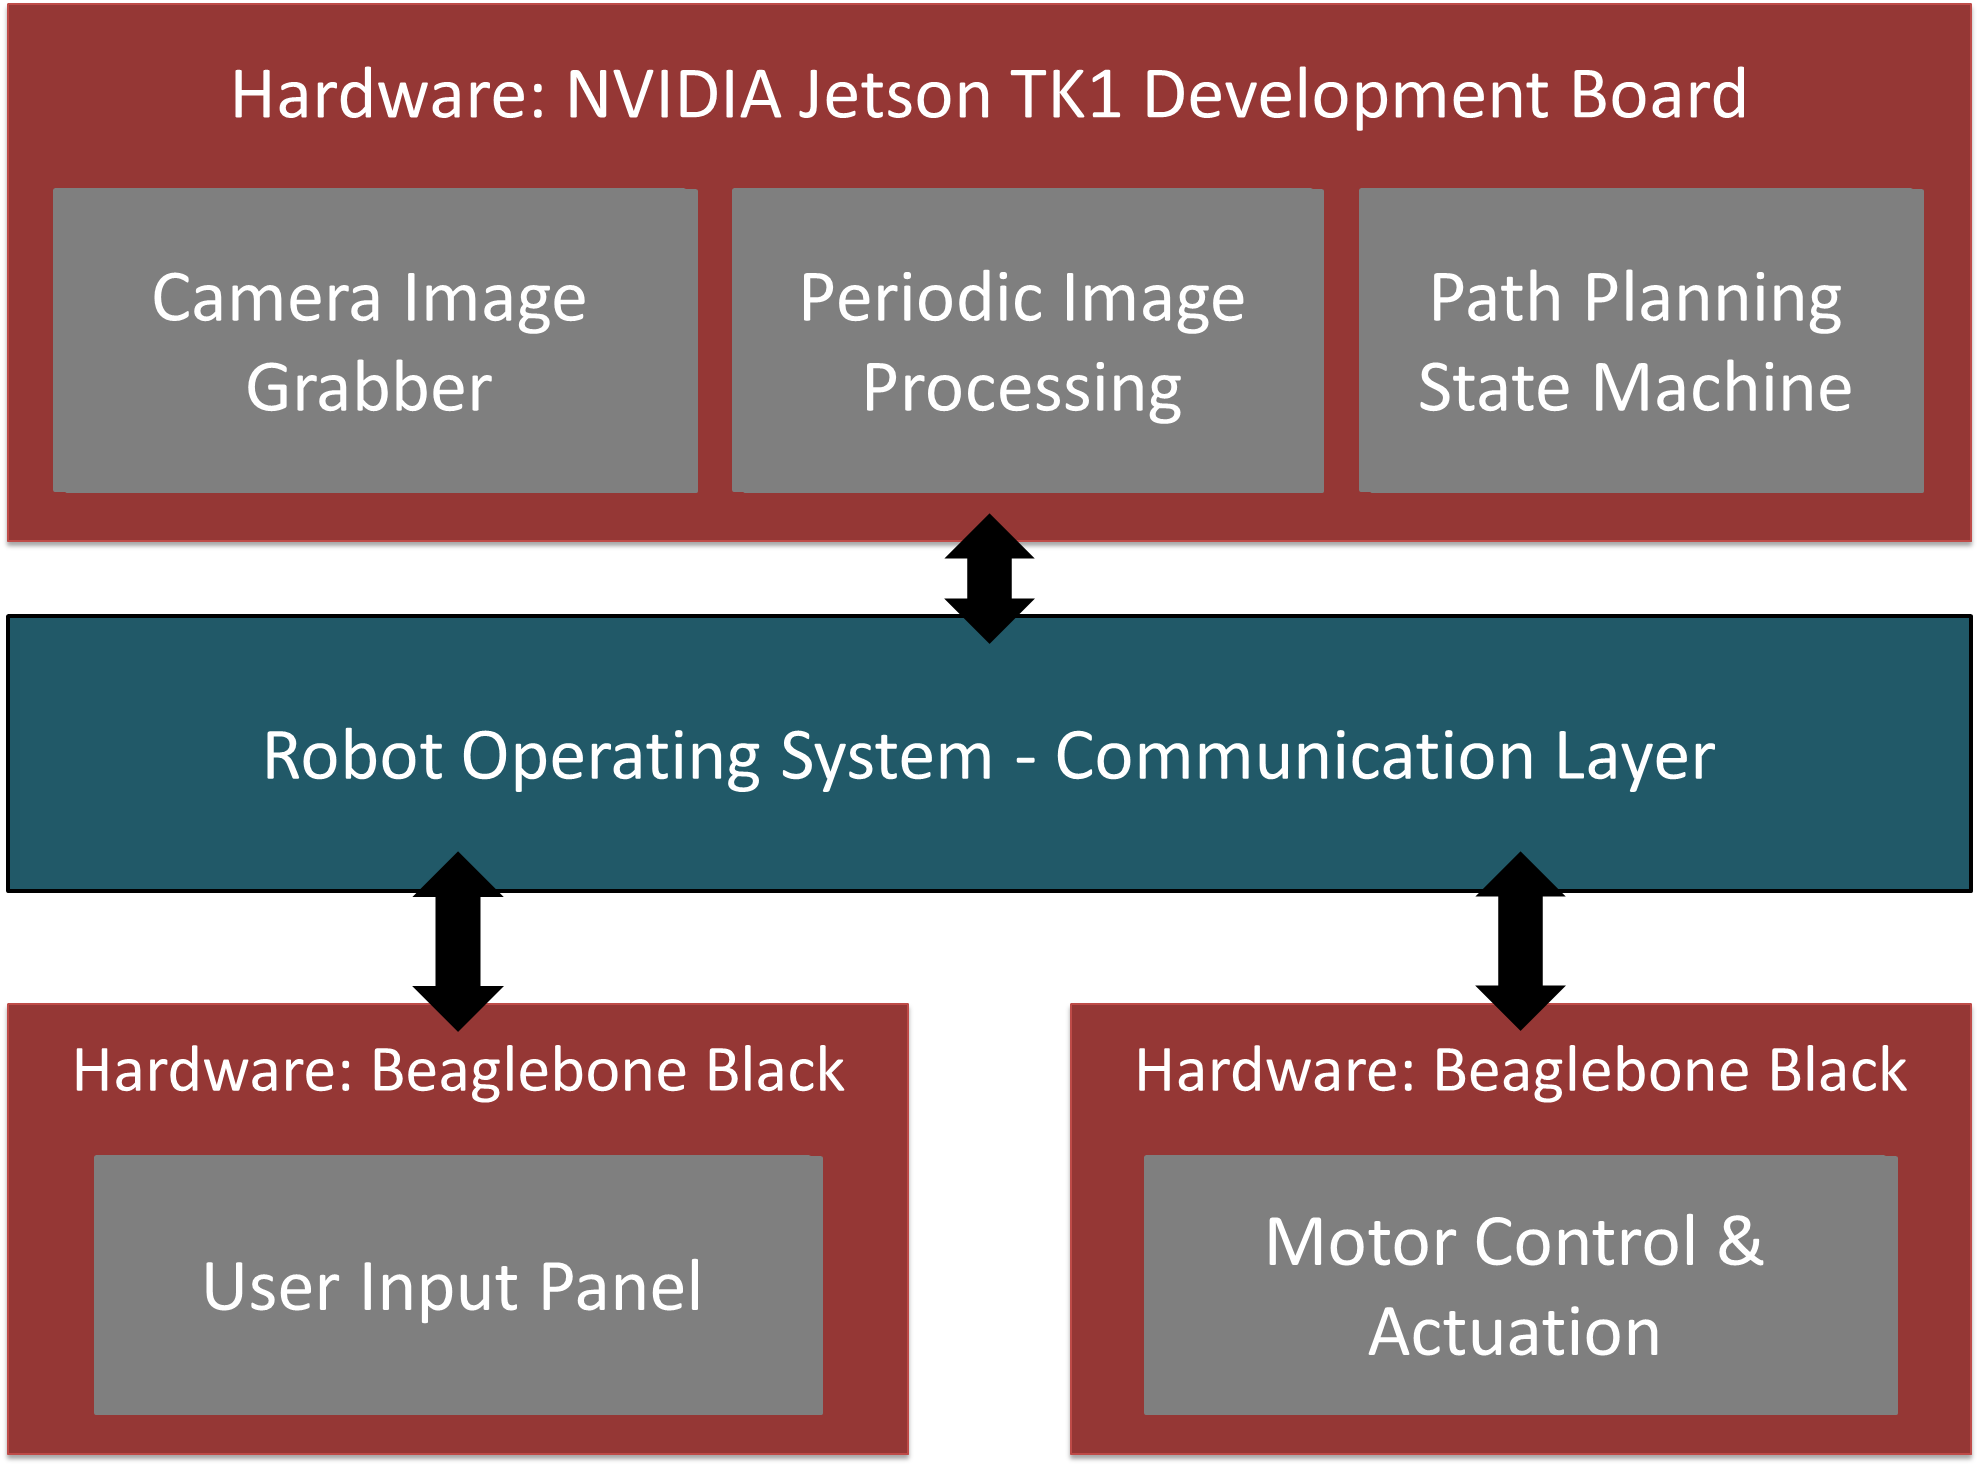
\includegraphics[width=0.45\textwidth]{figs/AGSE_Deployment.png}
	\caption{AGSE Package Deployment}
	\label{fig:AGSE_Deployment}
\end{figure}

\begin{figure*}[t]
	\centering	
	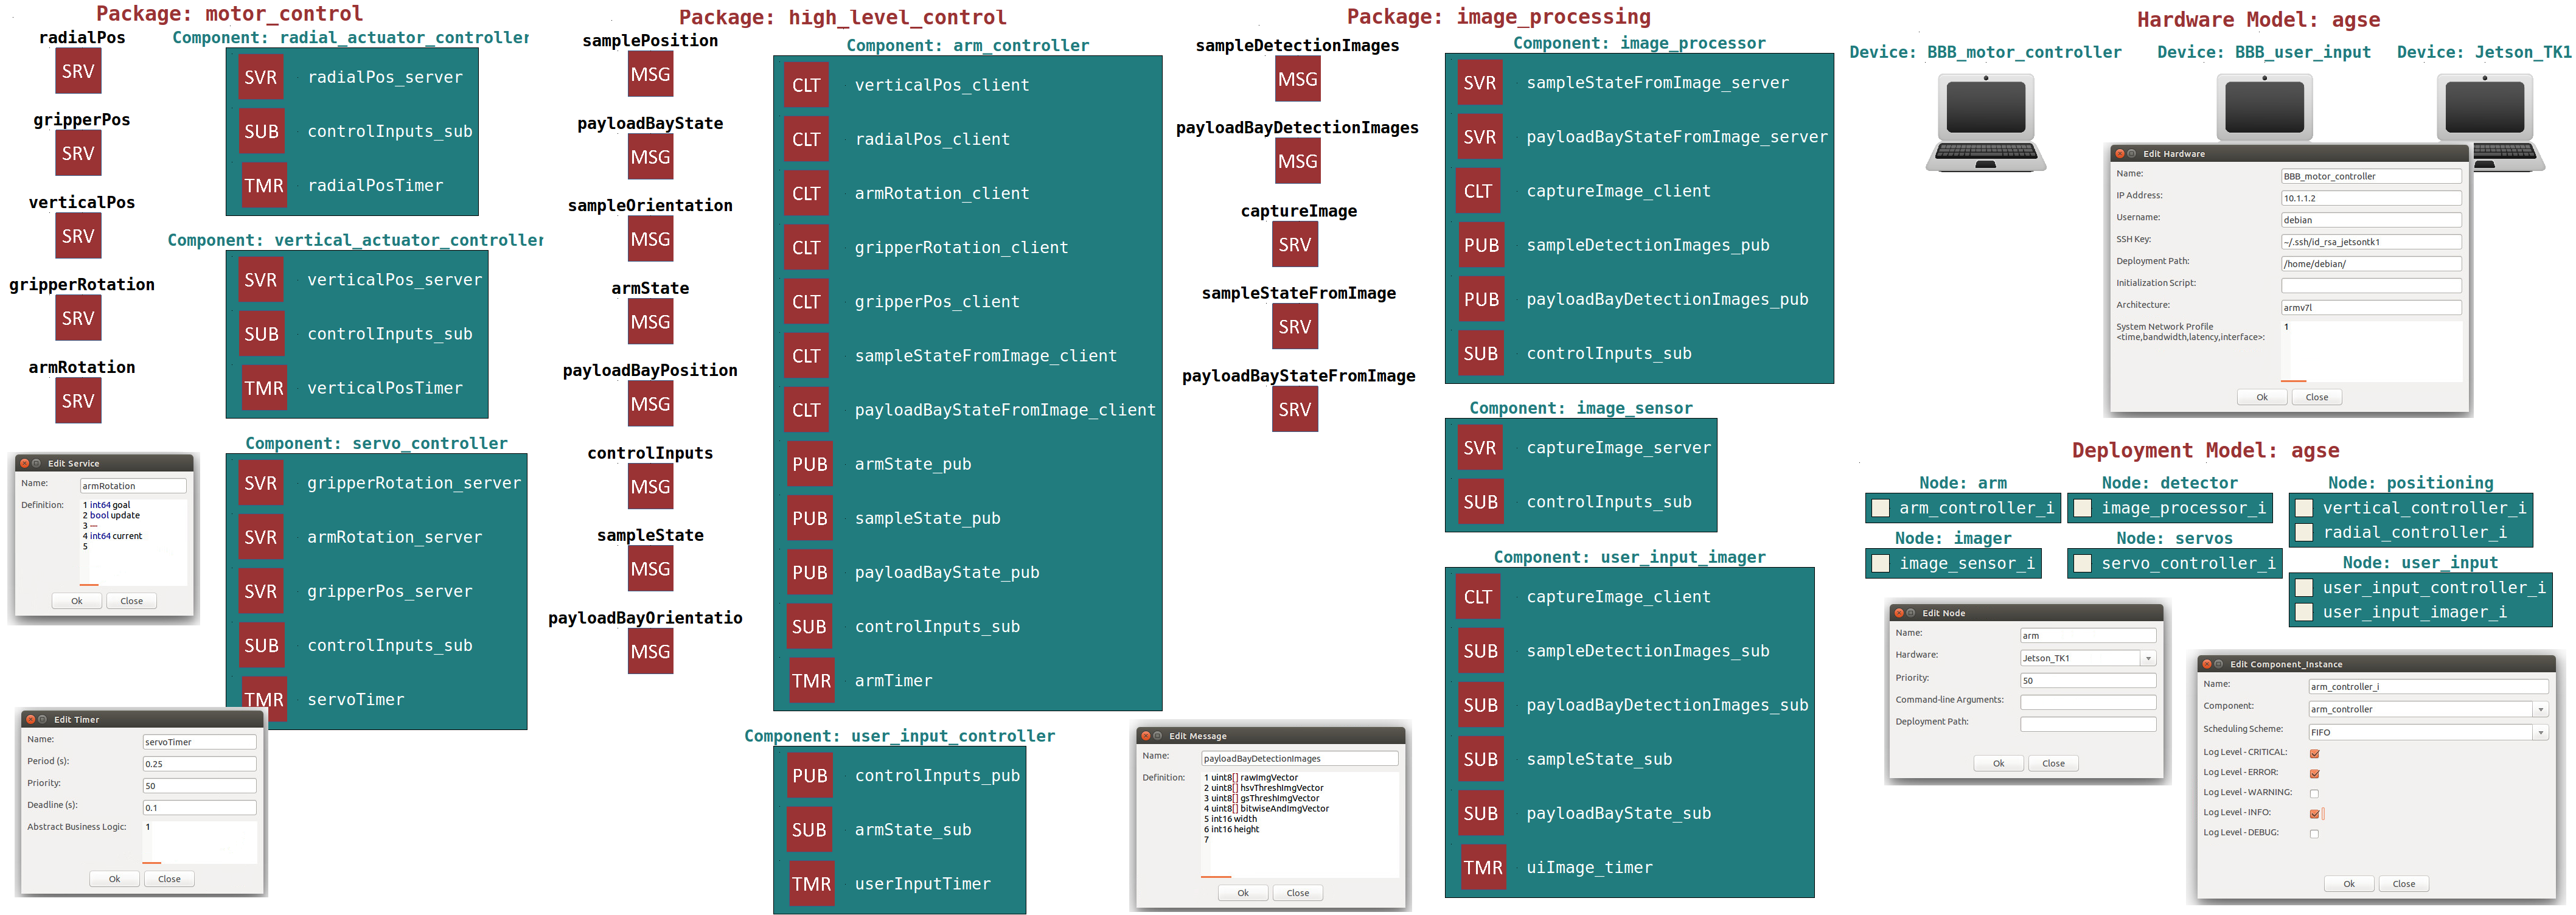
\includegraphics[width=1.0\linewidth]{figs/AGSE.png}
	\caption{AGSE ROSMOD Model}
	\label{fig:AGSE}	
\end{figure*}

An NVIDIA Jetson TK1 periodically fetches the latest webcam feed, performs image processing and high-level path planning, updating a global state machine. A Beaglebone black (BBB) mounted on top of the robot performs power management, low-level motor control and feedback processing. Lastly, a \emph{User Input Panel} houses a second Beaglebone Black, reacting to user input e.g. pause switch, touchscreen mode changes etc. This last controller is also responsible for keeping the user informed about the real-time state of the AGSE and the current webcam feed. Each of these controllers host ROS multiple nodes with ROSMOD component executor threads periodically performing algorithmic computations, calculating new robotic paths and maintaining the global state machine.


\subsubsection{Image Processing and Path Planning}

Periodic sample detection performed by the AGSE uses OpenCV-based image processing algorithms to identify and track the sample in real-time. An Image Processor component periodically fetches the latest feed from the mounted camera and performs a series of filtering tasks. 

Each \emph{RGB} image frame is converted to both \emph{HSV} (hue-saturation-value) and \emph{Grayscale} image frames. After applying thresholds, filters, erosion and dilation methods, the target sample is extracted from the webcam feed. Once the target sample is detected, we draw contours around the object and identify its relative position and orientation. Figures \ref{fig:Sample_Image_Processing} and \ref{fig:Sample_Image_Processing_2} present our launch-day results.

\subsubsection{Motor Control}
%Low-Level motor control: Servo control scheme: move to given position, tuned PID gains, dc motors controlled via H-bridges on motor board


%\subsubsection{User Input}
%Pause functionality, touch panel...

%\subsection{Fabrication and Procurement}
%fabrication methods and vendors for mechanical system, pcb's, COTS items, mention BOM in github repo?


\subsection{Software Prototyping with ROSMOD}

The AGSE software \cite{AGSE} was iteratively designed and rapid prototyped using ROSMOD. Figure \ref{fig:AGSE} shows the fully constructed ROSMOD models for the AGSE. The Software Model consists of 8 components spread across three ROS packages - motor control, high-level state machine control and image processing. Each package is characterized by its local set of messages, services and interacting components. 

The deployment model shows the various ROS nodes in the final system. Each node instantiates one or more components defined in the Software model e.g. the \emph{positioning} node executes two component threads, one behaving as a vertical\_actuator\_controller component and the other behaving as a radial\_actuator\_controller component. Each of these nodes is then deployed on one of the hardware devices modeled in the hardware model.

The ROSMOD code generators enabled generation of nearly 60\% (6,000+ lines) of the total built code. As mentioned before, much of this code includes port initialization, build system files, callback skeletons, etc. that usually take up a significant amount of development time. As developers, we had to fill in the missing pieces - the business logic of the generated callbacks, completing the component interaction loops. This code includes architecture-specific control, e.g. GPIO and encoder readings, LED and switch settings, camera image acquisition, and high-level control.  


%----------------Results Section------------------------------


\subsection{Competition Performance Assessment}

At the competition, the Vanderbilt AGSE was able to complete the sample retrieval process in approximately $4.5$ minutes. The recovery process, as shown in Figure \ref{fig:AGSE_Operation}, was successful, with payload and rocket bay recognition occurring quickly and efficiently. The AGSE was able to grasp the payload using only two of its four padded end effector phalanges, and successfully deposited the payload within the rocket bay. This operation received high marks from the NASA officials and earned the competition's \emph{Autonomous Ground Support Equipment Award}.

\begin{figure}[t]
	\centering	
	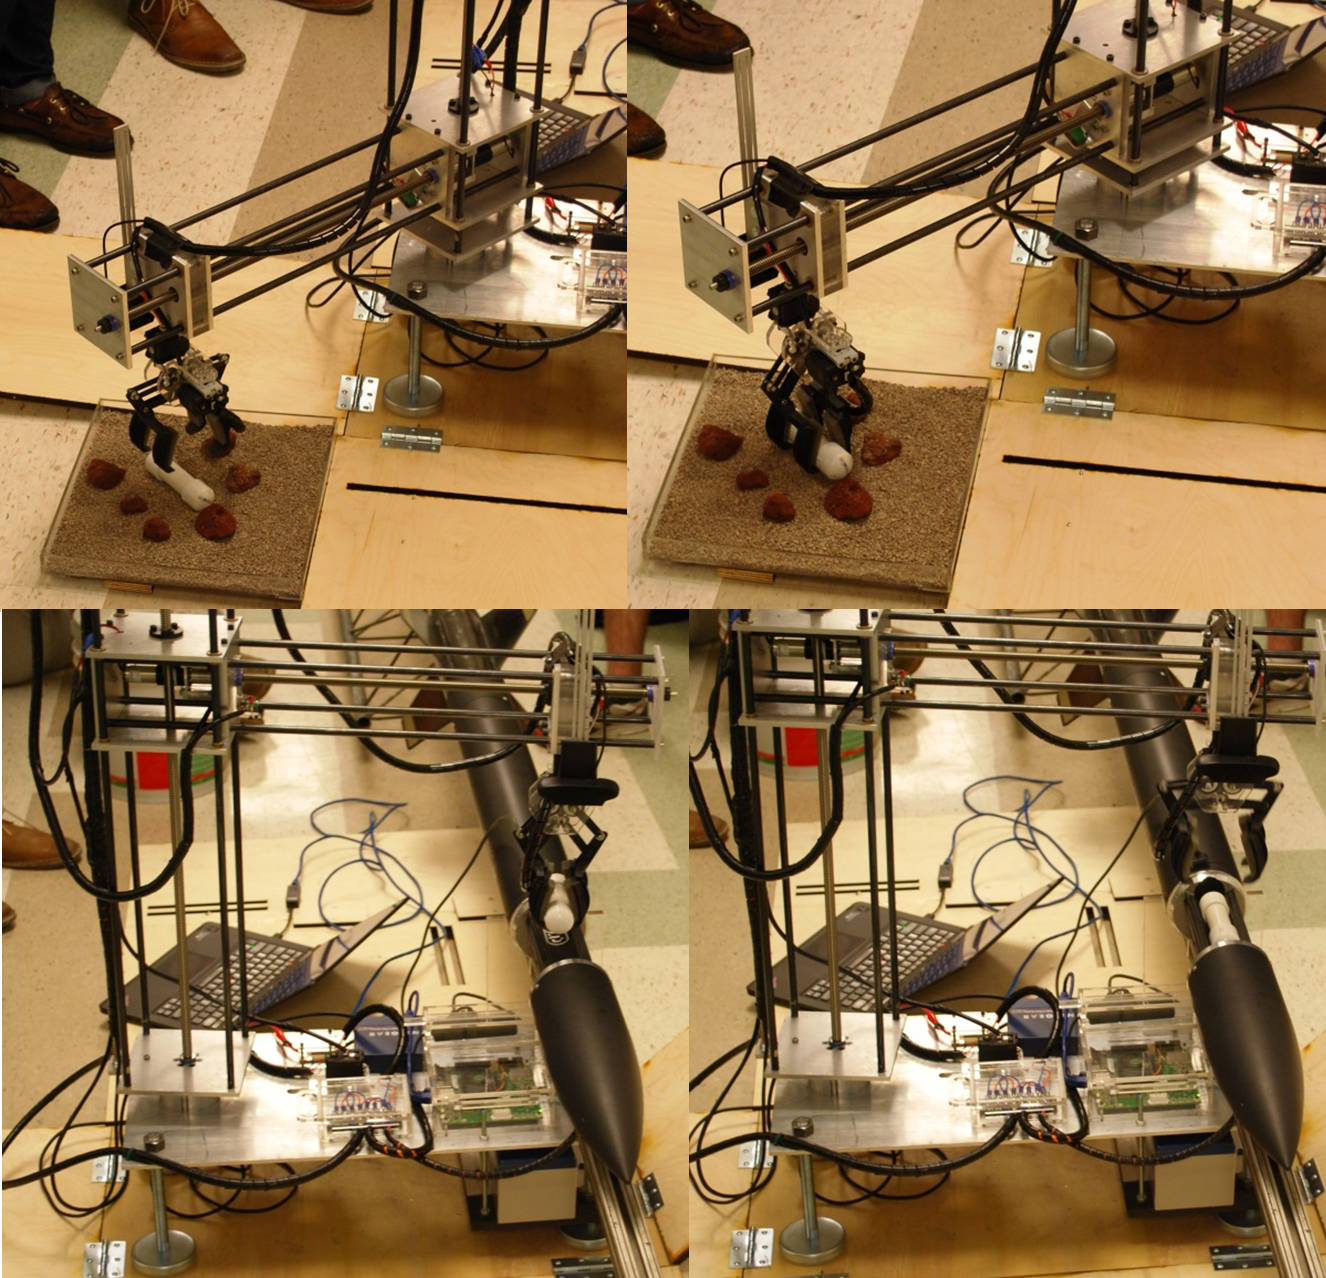
\includegraphics[width=1.0\linewidth]{figs/AGSE_Operation.png}
	\caption{AGSE Calibration and Testing}
	\label{fig:AGSE_Operation}	
\end{figure}

System robustness was validated on the day of competition when a key component failed and was able to be quickly replaced with a different part with no detriment to system performance. The Dynamixel AX-12A servo controlling the base rotational degree of freedom of the AGSE suffered an irreparable failure of its gearbox and had to be removed from the robot. A backup of the servo was not readily available, and a different model servo by the same company had to be swapped in instead.  This new model, a Dynamixel MX-28T, while having similar performance as the old servo, had a different communication protocol and mounting footprint, as well as a more complex control scheme.

The component-based nature of ROSMOD allowed quick modifications of the business logic of the \emph{servo\_controller} package to update the system to use the new hardware.  The new control scheme was quickly implemented and the new physical placement of the servo due to its different mounting footprint was accounted for in software. After these modifications were made, the AGSE was able to perform at its optimal level during its part of the competition.

The rapid prototyping facilitated by ROSMOD and the ROS infrastructure enabled the development of an overall \emph{smarter} robot. The software requirements for autonomy were matched by the ROSMOD code generators such that developers had to spend little time setting up the build system and interaction patterns. The speed of development was drastically improved and the \emph{business logic} code, i.e. the core of the implementation of the system behavior, could be made more robust.

\subsection{Post-Competition Testing and Performance}
